\documentclass{article}
\usepackage[utf8, margin=1.3in, top=1in, bottom=1in]{geometry}
\usepackage{pdfpages}

\title{Usability test report}
\author{Mikkel Aas \and Magnus Gluppe \and Jakob Frantzvåg Karlsmoen \and Mikael Falkenberg Krog}
\date{February 2020}


\begin{document}

\maketitle

\section{Introduction}
MetIma serves as an image gallery that allows the user to view the metadata of each image. We have conducted a usability test using wireframe. There were two participants; an observer and a participant. The observer captured the participants comments, navigational choices, task completion rate, comments, overall satisfaction rating, questions and feedback.

\subsection{Summary}
The most important findings were that our design was mostly intuitive, but a feature to import multiple images at the same time would be smart to include.

\subsection{Demographic}
We did not have enough time to perform usability testing with a large sample size. Since we do most of our work at the NTNU campus, we located a few other students to perform the usability test. Since our campus has a very homogeneous student body, the demographic we tested was males in their early 20's, with technological experience. This demographic is one that we expect to find great use in the application, as our application has a focus on image metadata.   

\subsection{Tasks}
The tasks the user had to perform were very basic navigational tasks, this was to see whether our application is intuitive. Since the test was performed using wireframe this was the only tasks our tester could do.
\section{Results}

\subsection{Usability Problems}
If the user were to upload thousands of images, our application could run into a problem with the gallery. The first model of wireframe uses a gallery which loads all the pictures when entering the gallery. This will use a lot of memory, and may cause the application to crash.
One major feature we lacked was the ability to import a folder of photos.

\subsection{Other Feedback}
We found that our application was highly intuitive, and was generally easy to use and understand. In the gallery we found that the focus should be on the tags, instead of the metadata. Furthermore, the search function should include the number of search results.
\newpage
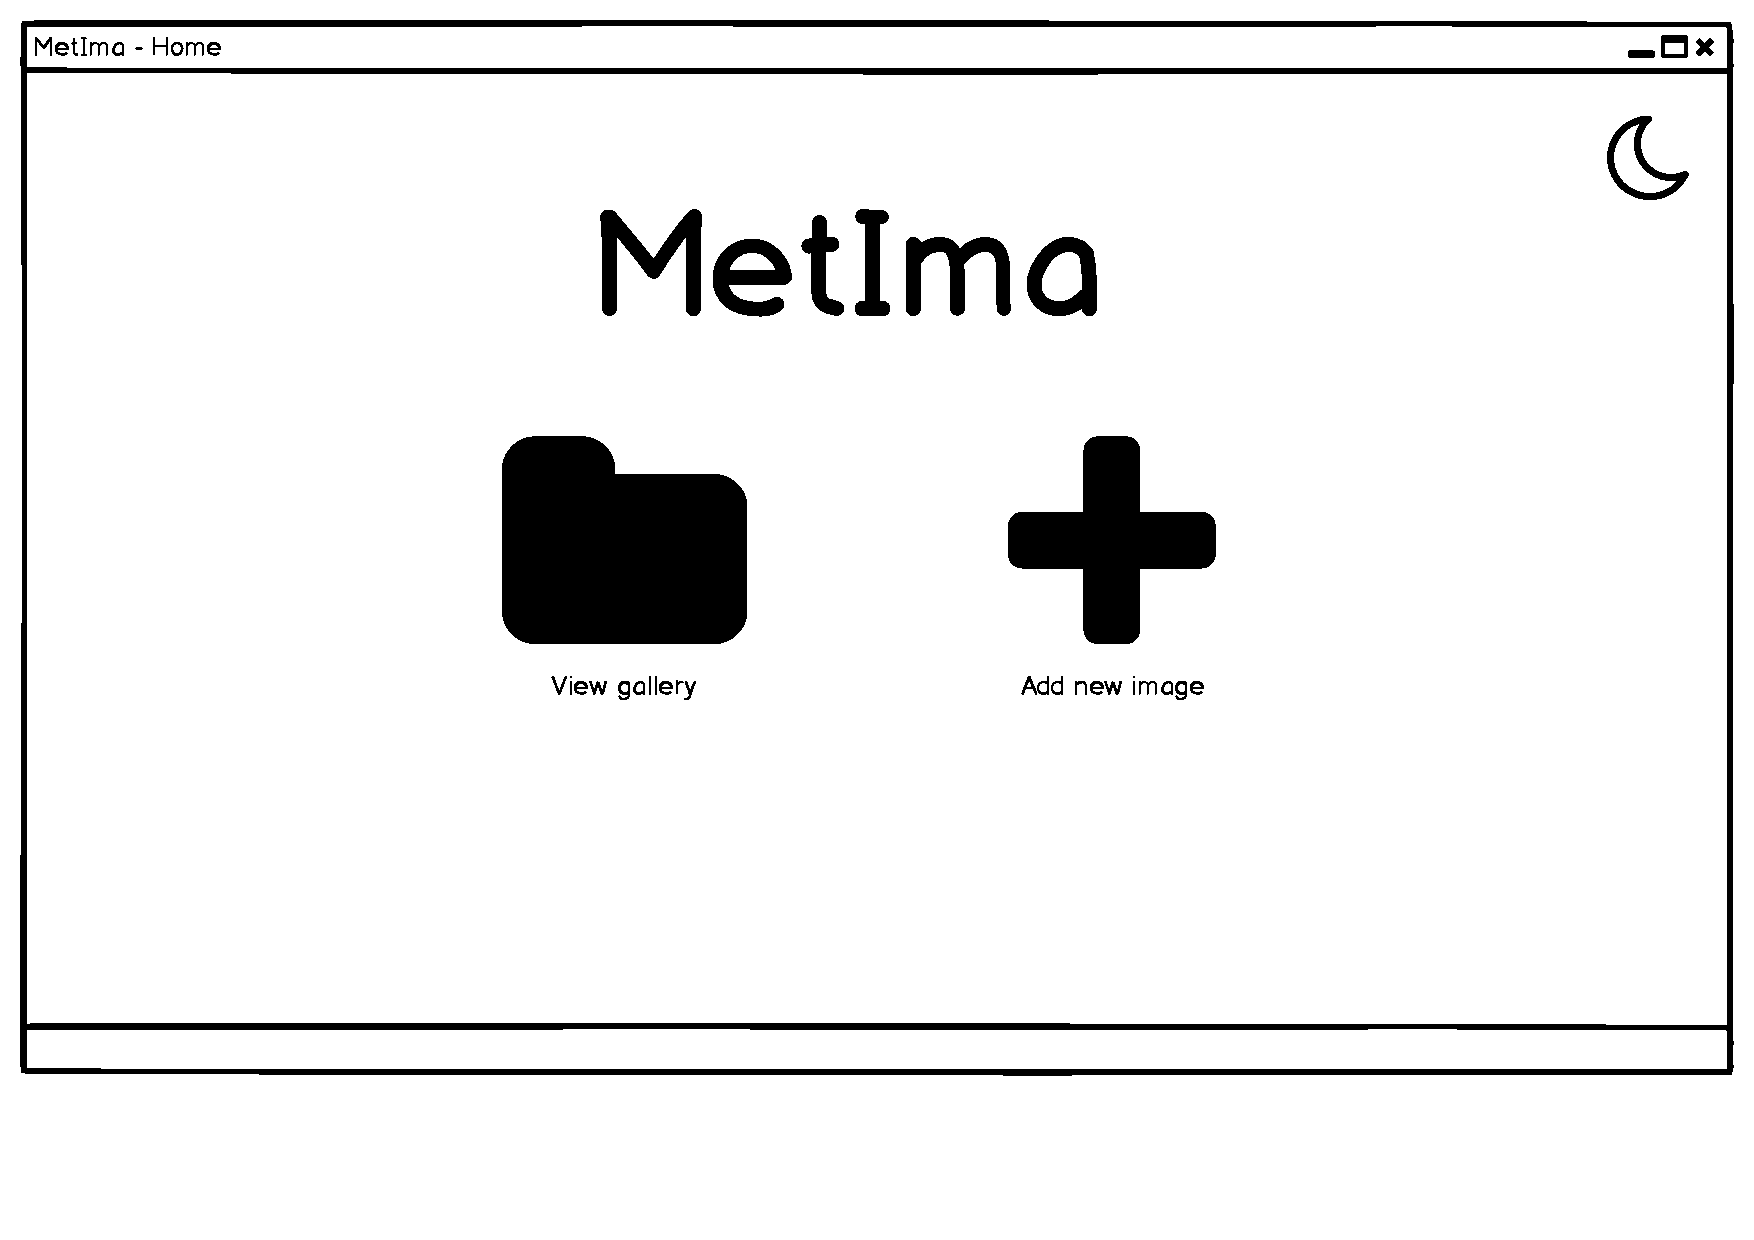
\includepdf[pages={1}, pagecommand=\section{Wireframe}]{Wireframe SUP.pdf}
\includepdf[pages={2,3,4}]{Wireframe SUP.pdf}
\end{document}